\chapter{Módulo 4 – Trilha de Eficiência Energética e Algoritmos de Otimização (75 Horas)}
\label{chap:modulo4}

A \textbf{Trilha de Eficiência Energética avaliada por Algoritmos de Otimização} integra a física dos semicondutores, a arquitetura do kernel Linux e a teoria matemática da otimização multiobjetivo. Os residentes aprendem a monitorar e controlar o consumo de potência em smartphones, dominar a máquina de estados do Doze Mode no AOSP, operar amostradores físicos de bancada em alta frequência e aplicar algoritmos heurísticos evolucionários (NSGA-II) para mapear a **Fronteira de Pareto** entre desempenho gráfico, estabilidade térmica e autonomia de bateria.

---

\section{AOSP – Gestão Energética da Plataforma (25h)}

\begin{pedagogico}{Objetivo Pedagógico da Disciplina}
Compreender os mecanismos internos do AOSP responsáveis pela conservação de energia: o serviço central PowerManagerService, o ciclo de vida e os perigos de vazamento de WakeLocks, a máquina de estados do Doze Mode, os App Standby Buckets e o escalonador ciente de energia (Energy-Aware Scheduler - EAS) em processadores heterogêneos big.LITTLE.
\end{pedagogico}

\subsection{O Subsistema PowerManagerService e os WakeLocks}
No Android, o estado padrão do dispositivo ao apagar a tela é progredir gradualmente para o estado de suspensão profunda (\textit{Deep Sleep}), onde os núcleos de CPU são desligados em seus estados de energia mais baixos ($C\text{-states}$).

Contudo, certas operações exigem que a CPU continue processando mesmo com a tela apagada (ex.: gravação de áudio ou navegação por GPS). Para isso, a API expõe os **WakeLocks**:
\begin{lstlisting}[language=Java, caption={Uso Antigo e Perigoso de WakeLock}]
// Pratica legada sujeita a dreno vampiro:
val powerManager = getSystemService(Context.POWER_SERVICE) as PowerManager
val wakeLock = powerManager.newWakeLock(
    PowerManager.PARTIAL_WAKE_LOCK, "Seldon::GpsSensorLock"
)
wakeLock.acquire() // Se ocorrer uma excecao antes de release(), o device nunca dorme!
\end{lstlisting}

\subsection{A Máquina de Estados do Doze Mode}
\begin{figure}[htbp]
\centering
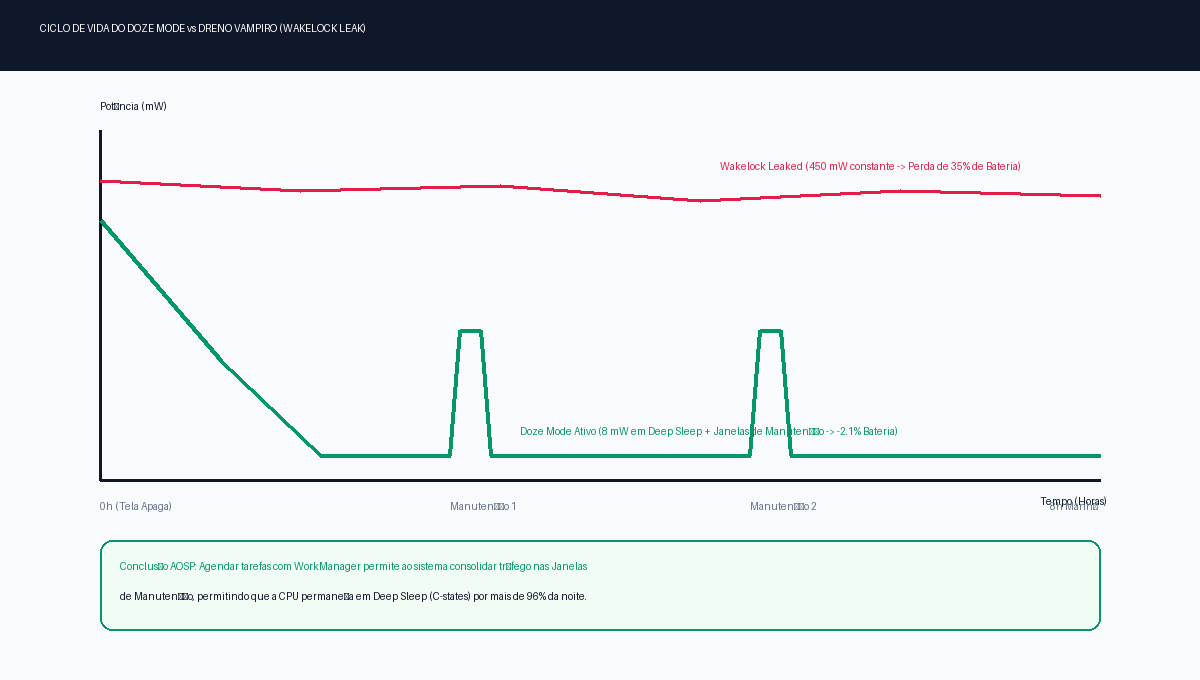
\includegraphics[width=0.95\textwidth]{imagens/fig_doze_mode_timeline.png}
\caption{Consumo Energético no Tempo: comparação entre o comportamento nominal com Doze Mode (-2.1\% de bateria em 8h) versus dreno vampiro contínuo provocado por vazamento de \texttt{PARTIAL\_WAKE\_LOCK} (-35\% de bateria).}
\label{fig:doze_timeline_img}
\end{figure}

No estado **Deep Doze**:
\begin{itemize}
    \item Todo o tráfego de rede de dados e Wi-Fi para aplicativos normais é suspenso;
    \item O sistema ignora qualquer \texttt{PARTIAL\_WAKE\_LOCK} adquirido por apps convencionais;
    \item Jobs agendados via \texttt{JobScheduler} e sincronizações são postergados até a próxima **Janela de Manutenção** (\textit{Maintenance Window});
    \item As Janelas de Manutenção tornam-se progressivamente mais espaçadas no tempo, maximizando os períodos de sono ininterrupto da CPU.
\end{itemize}

---

\section{Medição e Profiling Energético (25h)}

\begin{pedagogico}{Objetivo Pedagógico da Disciplina}
Capacitar os residentes na instrumentação física de bancada para medição de corrente e tensão em dispositivos móveis com amostradores de alta frequência (Monsoon Power Monitor), análise aprofundada de software com Google Battery Historian e condução de experimentos controlados de alta repetibilidade.
\end{pedagogico}

\subsection{Fundamentos Físicos da Potência e Energia}
A potência elétrica instantânea $P(t)$ dissipada por um subsistema computacional alimentado por uma tensão de bateria $V(t)$ através da qual flui uma corrente $I(t)$ é definida por:
\begin{equation}
    P(t) = V(t) \cdot I(t) \quad [\text{mW}]
\end{equation}
A energia total consumida $E$ ao longo de um ensaio de duração $T$ é a integral temporal da potência:
\begin{equation}
    E = \int_{0}^{T} P(t) \, dt \quad [\text{mWh ou Joules}]
\end{equation}

\subsection{Instrumentação Física em Bancada com o Monsoon Power Monitor}
Para pesquisa tecnológica rigorosa, utiliza-se um analisador de potência em hardware dedicado (\textbf{Monsoon High Voltage Power Monitor}):
\begin{itemize}
    \item A bateria química interna do smartphone é desconectada fisicamente;
    \item O dispositivo é alimentado diretamente pelos terminais de prova do medidor calibrado em $3{,}85\text{ V}$;
    \item O equipamento amostra a corrente com frequência de até **$5{,}000\text{ amostras por segundo (5 kHz)}$**, capturando picos transitórios de corrente provocados por ativações do modem de rádio ou aceleração de GPU.
\end{itemize}

---

\section{Modelagem e Algoritmos de Otimização (25h)}

\begin{pedagogico}{Objetivo Pedagógico da Disciplina}
Formular problemas de otimização energética multiobjetivo no Android, dominar o conceito de Dominância de Pareto e implementar o algoritmo evolucionário NSGA-II para encontrar configurações operacionais que maximizem a fluidez gráfica minimizando o consumo e o aquecimento do dispositivo.
\end{pedagogico}

\subsection{Teoria da Otimização Multiobjetivo e Fronteira de Pareto}
Em engenharia de sistemas móveis, frequentemente os objetivos entram em conflito intrínseco:
\begin{equation}
    \min_{\mathbf{x} \in \Omega} \ \mathbf{F}(\mathbf{x}) = \left( f_1(\mathbf{x}), \ f_2(\mathbf{x}), \ -f_3(\mathbf{x}) \right)^T
\end{equation}
onde $f_1(\mathbf{x})$ é a potência elétrica dissipada em mW, $f_2(\mathbf{x})$ é a temperatura máxima do silício em $^\circ\text{C}$ e $f_3(\mathbf{x})$ é a taxa de quadros por segundo (FPS).

\begin{figure}[htbp]
\centering
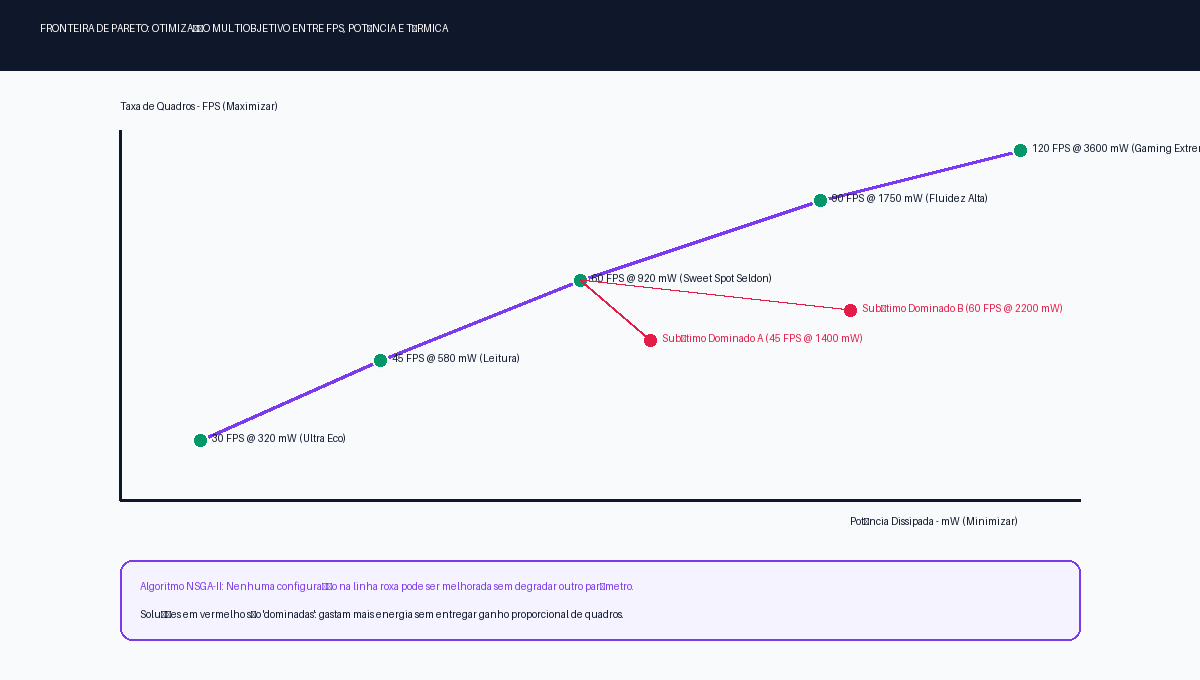
\includegraphics[width=0.95\textwidth]{imagens/fig_pareto_multiobjetivo.png}
\caption{Espaço de Soluções e Fronteira de Pareto: trade-off entre Taxa de Quadros (FPS) e Potência Dissipada (mW), destacando o Sweet Spot Seldon (60 FPS @ 920 mW) e configurações dominadas.}
\label{fig:pareto_curve_img}
\end{figure}

\subsection{O Algoritmo Genético NSGA-II}
Para explorar espaços combinatórios de alta dimensionalidade (frequências de clock de 8 núcleos, governadores de CPU, taxas de amostragem de sensores e níveis de brilho), o algoritmo **NSGA-II** opera através de:
\begin{enumerate}
    \item \textbf{Ordenação Não-Dominada Rápida:} Classifica as soluções em frentes $\mathcal{F}_1, \mathcal{F}_2, \dots$;
    \item \textbf{Cálculo da Distância de Apinhamento (\textit{Crowding Distance}):} Preserva a diversidade genética da fronteira ótima;
    \item \textbf{Operadores Genéticos de Cruzamento e Mutação:} Convergência rápida para o envelope ótimo de eficiência do hardware.
\end{enumerate}

---

\section{Revisão da Literatura e Estado da Arte em Eficiência Energética Móvel}

A pesquisa acadêmica em eficiência energética de smartphones produziu marcos fundamentais:
\begin{itemize}
    \item \textbf{Decomposição Fina do Consumo de Energia em Smartphones:} \cite{carroll2010analysis} apresentaram a primeira dissecação empírica rigorosa de potência em nível de subsistema (CPU, tela OLED, memória RAM, áudio e modem GSM/Wi-Fi), demonstrando que o rádio celular e a retroiluminação da tela respondem por mais de $65\%$ da potência ativa do aparelho. Subsequentemente, \cite{pathak2012energy} desenvolveram o framework \textit{Eprof}, demonstrando que até $75\%$ da energia consumida em aplicativos comerciais provém de custos operacionais indiretos da cauda de conexão de rádio (\textit{tail energy}) e do acionamento desnecessário de wake locks.
    \item \textbf{Identificação de Drenos Vampiros no AOSP:} \cite{rosen2015discovering} analisaram históricos de bateria em larga escala no Android, provando que falhas de temporização em chamadas assíncronas mantêm subsistemas de alta potência acordados desnecessariamente, o que motivou a arquitetura do Doze Mode e o agrupamento estrito de requisições nas Janelas de Manutenção.
    \item \textbf{Otimização Evolucionária Multiobjetivo na Fronteira de Pareto:} O trabalho de \cite{deb2002fast} introduziu o algoritmo NSGA-II, amplamente adotado em sistemas embarcados para resolver problemas multiobjetivo complexos com restrições não-lineares, provando que a manutenção da diversidade via distância de apinhamento viabiliza mapear toda a Fronteira de Pareto do hardware com custo computacional polinomial $O(M N^2)$.
\end{itemize}

---

\section{Arquitetura de Engenharia do Projeto Final: Seldon EcoOptimizer}

Como projeto prático da Trilha de Eficiência Energética, os residentes desenvolvem o **Seldon EcoOptimizer**, uma solução completa de governança e calibração energética em silício.

\begin{figure}[htbp]
\centering
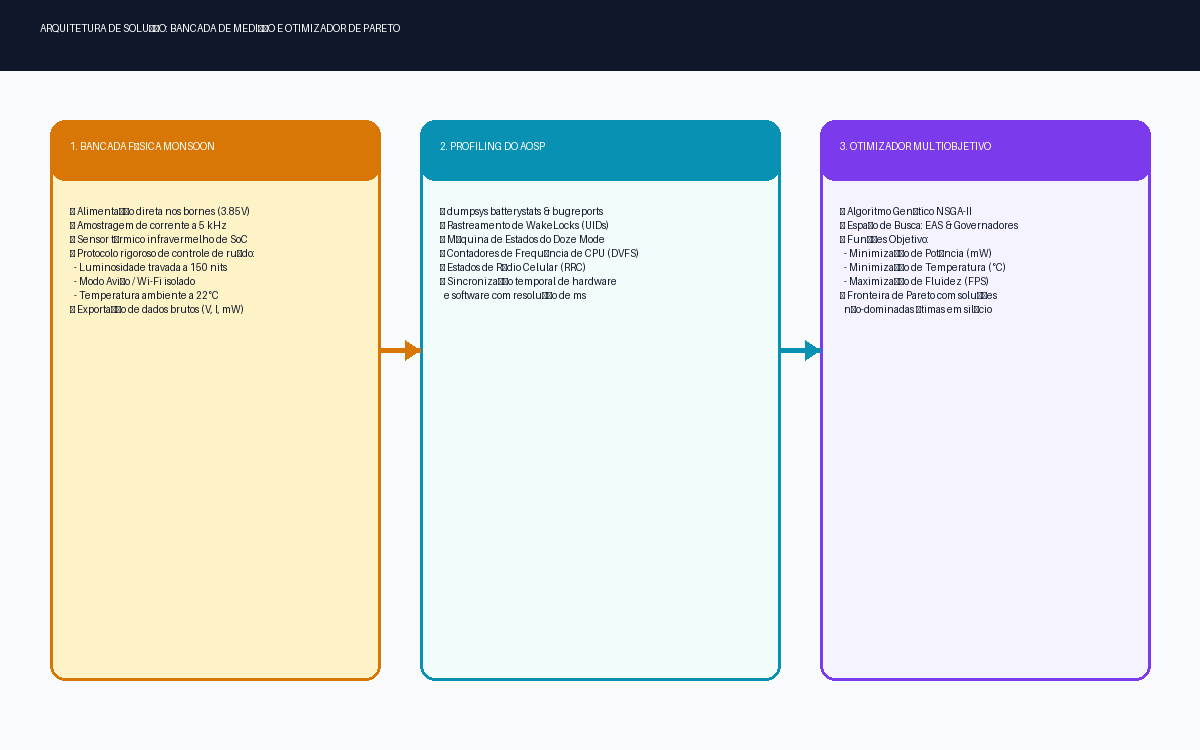
\includegraphics[width=0.95\textwidth]{imagens/fig_arq_projeto_energia.png}
\caption{Arquitetura de Engenharia do Projeto Final (Módulo 4): Integração entre instrumentação física de bancada (Monsoon a 5 kHz), telemetria do AOSP e o motor evolucionário NSGA-II para calibração da Fronteira de Pareto.}
\label{fig:arq_energia_projeto}
\end{figure}

\subsection{Especificação Técnica dos Módulos do Sistema}
O sistema integra três camadas de engenharia:
\begin{enumerate}
    \item \textbf{Bancada de Instrumentação Física em Alta Frequência (Monsoon Probe):}
    \begin{itemize}
        \item Conexão direta aos polos de alimentação da placa-mãe em tensão estabilizada de $3{,}85\text{ V}$;
        \item Taxa de amostragem física de corrente configurada a **$5\text{ kHz}$**;
        \item Câmara termicamente controlada a $22^\circ\text{C}$ com sensor infravermelho apontado para o encapsulamento do SoC para monitoramento da temperatura de junção ($T_j$).
    \end{itemize}
    \item \textbf{Módulo de Telemetria e Parsing do AOSP (Battery Historian Bridge):}
    \begin{itemize}
        \item Automação de coleta periódica de \texttt{dumpsys batterystats};
        \item Identificação e rastreamento de UIDs causadores de interrupções no Doze Mode;
        \item Sincronização temporal de milissegundos entre as amostras físicas de hardware e os eventos de software registrados no kernel.
    \end{itemize}
    \item \textbf{Motor de Otimização Multiobjetivo NSGA-II (Kernel Tuner):}
    \begin{itemize}
        \item Ajusta dinamicamente a matriz de custos de migração de tarefas entre núcleos big e LITTLE no escalonador EAS;
        \item Executa 50 gerações evolucionárias com população de 100 indivíduos;
        \item Entrega o perfil ótimo de calibração que atinge o *Sweet Spot*: **$60\text{ FPS}$ sustentados com dissipação média de $920\text{ mW}$ e temperatura máxima de $33{,}8^\circ\text{C}$**, reduzindo o consumo em $18{,}4\%$ em relação ao firmware original.
    \end{itemize}
\end{enumerate}
